\documentclass[tikz,border=2pt]{standalone}
\usepackage{amsmath}
\usepackage{pgfplots}
\pgfplotsset{compat=1.18}
\usetikzlibrary{arrows.meta}
\begin{document}
% Left: the concave upper semicircle f(x)=sqrt(1-x^2) on [-1,1]; its hypograph (unbounded below) is convex.
% Right: the convex x^2; (-1,1) and (1,1) lie in Hypo(x^2) but their midpoint (0,1) does not, since 0<1.
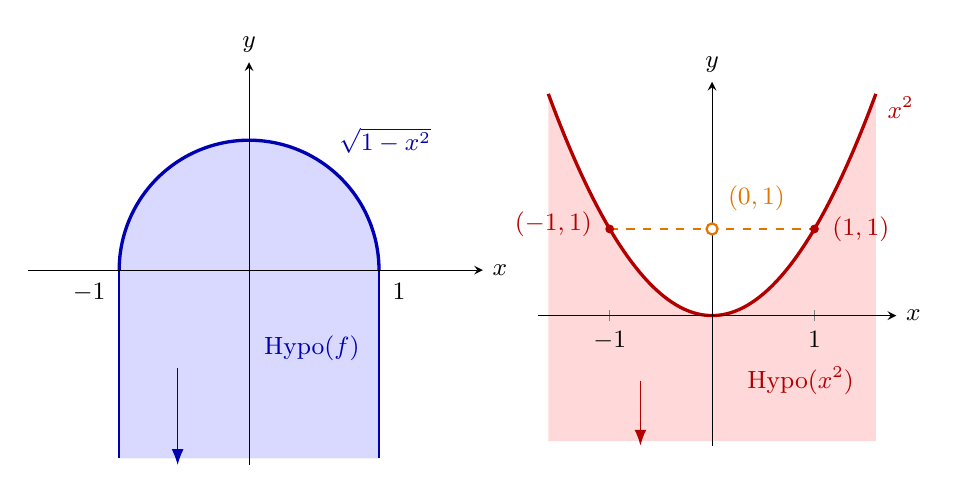
\begin{tikzpicture}[font=\small, >={Latex[length=2mm]}]
  \begin{axis}[
    name=left, axis lines=middle, axis on top, xmin=-1.7, xmax=1.8, ymin=-1.5, ymax=1.6,
    xtick=\empty, ytick=\empty,
    xlabel={$x$}, ylabel={$y$},
    xlabel style={anchor=west}, ylabel style={anchor=south},
    x=1.65cm, y=1.65cm, clip=false
    ]
    \addplot[draw=none, fill=blue!15, domain=0:180, samples=90] ({cos(x)},{sin(x)}) -- (axis cs:-1,-1.45) -- (axis cs:1,-1.45) -- cycle;
    \draw[blue!70!black, thick] (axis cs:-1,0) -- (axis cs:-1,-1.45);
    \draw[blue!70!black, thick] (axis cs:1,0) -- (axis cs:1,-1.45);
    \addplot[blue!70!black, very thick, domain=0:180, samples=90] ({cos(x)},{sin(x)});
    \node[blue!70!black, anchor=south west] at (axis cs:0.62,0.82) {$\sqrt{1-x^2}$};
    \node[anchor=north east] at (axis cs:-1.03,-0.03) {$-1$};
    \node[anchor=north west] at (axis cs:1.03,-0.03) {$1$};
    \node[blue!70!black, anchor=west] at (axis cs:0.04,-0.6) {$\operatorname{Hypo}(f)$};
    \draw[blue!70!black, ->] (axis cs:-0.55,-0.75) -- (axis cs:-0.55,-1.5);
  \end{axis}
  \begin{axis}[
    at={(left.east)}, anchor=west, xshift=0.7cm,
    axis lines=middle, axis on top, xmin=-1.7, xmax=1.8, ymin=-1.5, ymax=2.7,
    xtick={-1,1}, ytick=\empty,
    xlabel={$x$}, ylabel={$y$},
    xlabel style={anchor=west}, ylabel style={anchor=south},
    x=1.3cm, y=1.1cm, clip=false,
    after end axis/.code={\filldraw[fill=white, draw=orange!90!black, thick] (axis cs:0,1) circle (2pt);}
    ]
    \addplot[draw=none, fill=red!15, domain=-1.6:1.6, samples=80] {x^2} -- (axis cs:1.6,-1.45) -- (axis cs:-1.6,-1.45) -- cycle;
    \addplot[red!70!black, very thick, domain=-1.6:1.6, samples=80] {x^2};
    \node[red!70!black, anchor=west] at (axis cs:1.62,2.4) {$x^2$};
    \node[red!70!black, anchor=west] at (axis cs:0.25,-0.75) {$\operatorname{Hypo}(x^2)$};
    \draw[red!70!black, ->] (axis cs:-0.7,-0.75) -- (axis cs:-0.7,-1.5);
    \draw[orange!90!black, thick, dashed] (axis cs:-1,1) -- (axis cs:1,1);
    \fill[red!70!black] (axis cs:-1,1) circle (1.6pt);
    \fill[red!70!black] (axis cs:1,1) circle (1.6pt);
    \node[red!70!black, anchor=east] at (axis cs:-1.08,1.05) {$(-1,1)$};
    \node[red!70!black, anchor=west] at (axis cs:1.08,1.0) {$(1,1)$};
    \node[orange!90!black, anchor=south west] at (axis cs:0.06,1.1) {$(0,1)$};
  \end{axis}
\end{tikzpicture}
\end{document}
